% Pillar 1 iter85 -- three-phase hypothesis (arXiv:2507.18014) test and
% Nemotron-120B collapse-signature audit.
\paragraph{Iter 85 elevation: the three-phase hypothesis survives the AIC
battery better than the saturation law, and the Nemotron-120B collapse is
its sharpest counter-example.}
\label{par:scaling-iter85}

iter 73 falsified the saturation law
$R(t) = R_\mathrm{max} \cdot (1 - e^{-\lambda t})$ as the universal family
across 12 anchors (AIC winner 2/12); iter 77 sharpened the falsification
with prefix-only fit and suffix-holdout $R^2$; iter 81 went further,
showing that the zero-mean constant model beats every 2-parameter family
on 11/12 single-axis strata and that the operational $k_{50}/k_{80}$
horizon is empty.  The remaining question was whether the canonical
\emph{three-phase} template (creep $\to$ spurt $\to$ level) of
Nimmaturi et al.\ (arXiv:2507.18014) does any better.  iter 85 fits a
3-segment piecewise-linear model with two greedy $O(n^2)$ changepoints
per anchor and scores it against 1-segment (slope+intercept) and
2-segment baselines.

\paragraph{Three-phase conformity: AIC improvement on 6/12 anchors, but
the canonical ordering survives almost everywhere.}
\label{par:scaling-iter85-conformity}

On the 9 anchors with at least $n \ge 10$ reward samples, the 3-segment
model beats the 1-segment AIC by $\Delta\mathrm{AIC}_{3\to 1} < -2$ in
\textbf{6/9} cases (Qwen3.5-4B $-4.65$, Qwen3-8B $-2.02$,
Llama-3.1-8B-Instruct $-6.26$, DeepSeek-V3.1 $-8.46$, Nemotron-120B
$-7.82$, Kimi-K2-Thinking $-2.81$).  This is a \emph{strict improvement}
over iter 73's saturation law, which only won 2/12 anchors under AIC.
The canonical temporal ordering (creep first, spurt in the middle, level
last) is preserved on \textbf{12/12} anchors that admit a 3-segment fit;
the property that the middle segment carries the largest $|\mathrm{slope}|$
(spurt dominance) holds on \textbf{9/12} anchors; the monotone-plateau
property ($|\mathrm{slope}_\mathrm{level}| \le |\mathrm{slope}_\mathrm{creep}|$)
holds on \textbf{8/12} anchors.  Four anchors reach a perfect 4-of-4
conformity score: Qwen3.5-4B, Qwen3-8B, Llama-3.1-8B-Instruct, and
Kimi-K2-Thinking.

\paragraph{Nemotron-120B collapse: a 3-phase trajectory whose spurt is
backwards.}
\label{par:scaling-iter85-nemotron}
Nemotron-120B's GSM8K reward trace reaches its peak reward $0.875$ at
\emph{step 3} and then collapses to $\mathrm{last10} = 0.163$, the most
extreme $\Delta = -0.713$ drop across the 12-anchor pool
(\tableref{tab:iter85-phases}).  The greedy 3-segment fit partitions the
trace as $[1\text{--}3] \cup [4\text{--}18] \cup [19\text{--}20]$ with
slopes $(+0.4375, -0.0054, 0.000)$ -- the canonical \emph{spurt} is now
the \emph{first} segment, and the canonical \emph{level} sits at a low
plateau near $0.05$ rather than at a saturated reward ceiling.  The
trajectory still wins the AIC 3-vs-1 comparison by $-7.82$ (i.e.\ a
3-segment fit is much better than a single linear trend), but it
\emph{violates the canonical creep-then-spurt ordering}: the creep phase
is missing entirely, the spurt is at $t=3$, and the level is at the
bottom of the reward range.  The conformance score of $3/4$ -- missing
only the monotone-plateau criterion because the final segment has zero
slope at a low value rather than at a saturated ceiling -- is a
signature of \emph{premature saturation followed by collapse} rather
than of the canonical three-phase learning template.  By contrast, the
other two anchors that violate the template (DeepSeek-V3.1 conform
$3/4$, gpt-oss-20B conform $2/4$) do so for a milder reason: their
spurt is not the largest-$|\mathrm{slope}|$ segment, but the changepoint
geometry is otherwise canonical.

\paragraph{Summary of iter 85 deliverables.}
\label{par:scaling-iter85-deliverables}

\begin{itemize}
    \item \texttt{scripts/scaling\_law\_iter85.py} ($\sim$300 lines,
        stdlib+numpy+matplotlib; greedy $O(n^2)$ piecewise-linear
        changepoint fit, AIC scoring, conformity audit, collapse
        diagnostics, 4-panel figure).
    \item 4 TSV outputs: \texttt{scaling\_law\_iter85\_phases.tsv}
        (12 rows; phase label, peak step, collapse delta),\\
        \texttt{scaling\_law\_iter85\_conformity.tsv} (12 rows; 1-seg,
        2-seg, 3-seg SSE and AIC, conformity sub-scores),\\
        \texttt{scaling\_law\_iter85\_changepoints.tsv} (12 rows;
        changepoint locations, segment slopes, segment lengths),\\
        \texttt{scaling\_law\_iter85\_nemotron.tsv} (12 rows;
        collapse delta, recovery ratio, trailing variance ratio,
        monotone-decline run after peak).
    \item \texttt{experiments/results/scaling\_law\_iter85\_meta.json}
        (aggregate counts: $6/12$ AIC winners, $9/12$ spurt-larger,
        $12/12$ canonical order, $8/12$ monotone plateau, $4/12$
        perfect score, $3/4$ Nemotron).
    \item \texttt{figures/scaling\_law\_iter85.pdf|png} (4-panel:
        reward traces colored by conformity score, AIC-$\Delta$
        horizontal bar, changepoint segment decomposition, Nemotron
        zoomed comparison vs the other 11 anchors).
\end{itemize}

\begin{table}[ht]
\centering
\small
\begin{tabular}{lrrrrr}
\hline
Anchor & $n$ & $\mathrm{first5}$ & $\mathrm{last10}$ &
$\mathrm{peak}$ & $\Delta_{\mathrm{last10}-\mathrm{peak}}$ \\
\hline
\rowcolor{green!10}
Qwen3.5-4B & 30 & 0.963 & 0.850 & 1.000 & $-0.150$ \\
\rowcolor{green!10}
Qwen3-8B & 30 & 0.312 & 0.344 & 0.625 & $-0.281$ \\
\rowcolor{green!10}
Llama-3.1-8B-Inst & 30 & 0.975 & 0.844 & 1.000 & $-0.156$ \\
Qwen3-32B & 3 & 0.250 & 0.250 & 0.312 & $-0.063$ \\
Qwen3.5-27B & 3 & 0.437 & 0.437 & 0.750 & $-0.313$ \\
gpt-oss-20B & 30 & 0.875 & 0.875 & 1.000 & $-0.125$ \\
Qwen3-30B-MoE & 5 & 0.325 & 0.325 & 0.500 & $-0.175$ \\
Qwen3-30B-MoE-Inst & 3 & 1.000 & 1.000 & 1.000 & $0.000$ \\
DeepSeek-V3.1 & 20 & 0.850 & 0.850 & 1.000 & $-0.150$ \\
\rowcolor{red!30}
Nemotron-120B & 20 & 0.175 & 0.163 & 0.875 & $\mathbf{-0.713}$ \\
Qwen3-235B-MoE & 4 & 1.000 & 1.000 & 1.000 & $0.000$ \\
Kimi-K2-Thinking & 20 & 0.925 & 0.800 & 1.000 & $-0.200$ \\
\hline
\end{tabular}
\caption{Pillar-1 iter-85 phase diagnostics across the 12-anchor pool.
Green: anchors that reach perfect 4/4 three-phase conformity.
Red: Nemotron-120B, the sharpest collapse signature
($\Delta_{\mathrm{last10}-\mathrm{peak}} = -0.713$, $\sim 4.7\times$
the median absolute collapse delta).}
\label{tab:iter85-phases}
\end{table}

\begin{table}[ht]
\centering
\small
\begin{tabular}{lrrrrrr}
\hline
Anchor & $\mathrm{SSE}_{1}$ & $\mathrm{SSE}_{3}$ &
$\Delta\mathrm{AIC}_{3\to 1}$ & spurtdom & canonord & conf$_4$ \\
\hline
Qwen3.5-4B & 1.39 & 0.85 & $-4.65$ & Y & Y & 4/4 \\
Qwen3-8B & 0.84 & 0.56 & $-2.02$ & Y & Y & 4/4 \\
Llama-3.1-8B-Inst & 0.77 & 0.45 & $-6.26$ & Y & Y & 4/4 \\
DeepSeek-V3.1 & 0.37 & 0.15 & $-8.46$ & N & Y & 3/4 \\
Nemotron-120B & 1.20 & 0.49 & $\mathbf{-7.82}$ & N & Y & 3/4 \\
Kimi-K2-Thinking & 0.48 & 0.25 & $-2.81$ & Y & Y & 4/4 \\
gpt-oss-20B & 1.09 & 0.78 & $-0.01$ & N & Y & 2/4 \\
\hline
\end{tabular}
\caption{Three-phase AIC and conformity scoring on the 7 anchors with
$n \ge 20$.  $\Delta\mathrm{AIC}_{3\to 1} < -2$ on \textbf{6/7}
indicates the 3-segment fit is the preferred parsimonious family --
stronger support than the saturation law's 2/12 in iter 73.  conf$_4$
is the count of 4 conformity sub-criteria met (3-phase AIC, spurt
largest $|\mathrm{slope}|$, canonical temporal order, monotone
plateau).  Nemotron-120B achieves 3/4: it satisfies the AIC criterion
and temporal order, but its spurt is the \emph{first} segment (peak at
step 3) rather than the middle one.}
\label{tab:iter85-conformity}
\end{table}

\begin{figure}[ht]
\centering
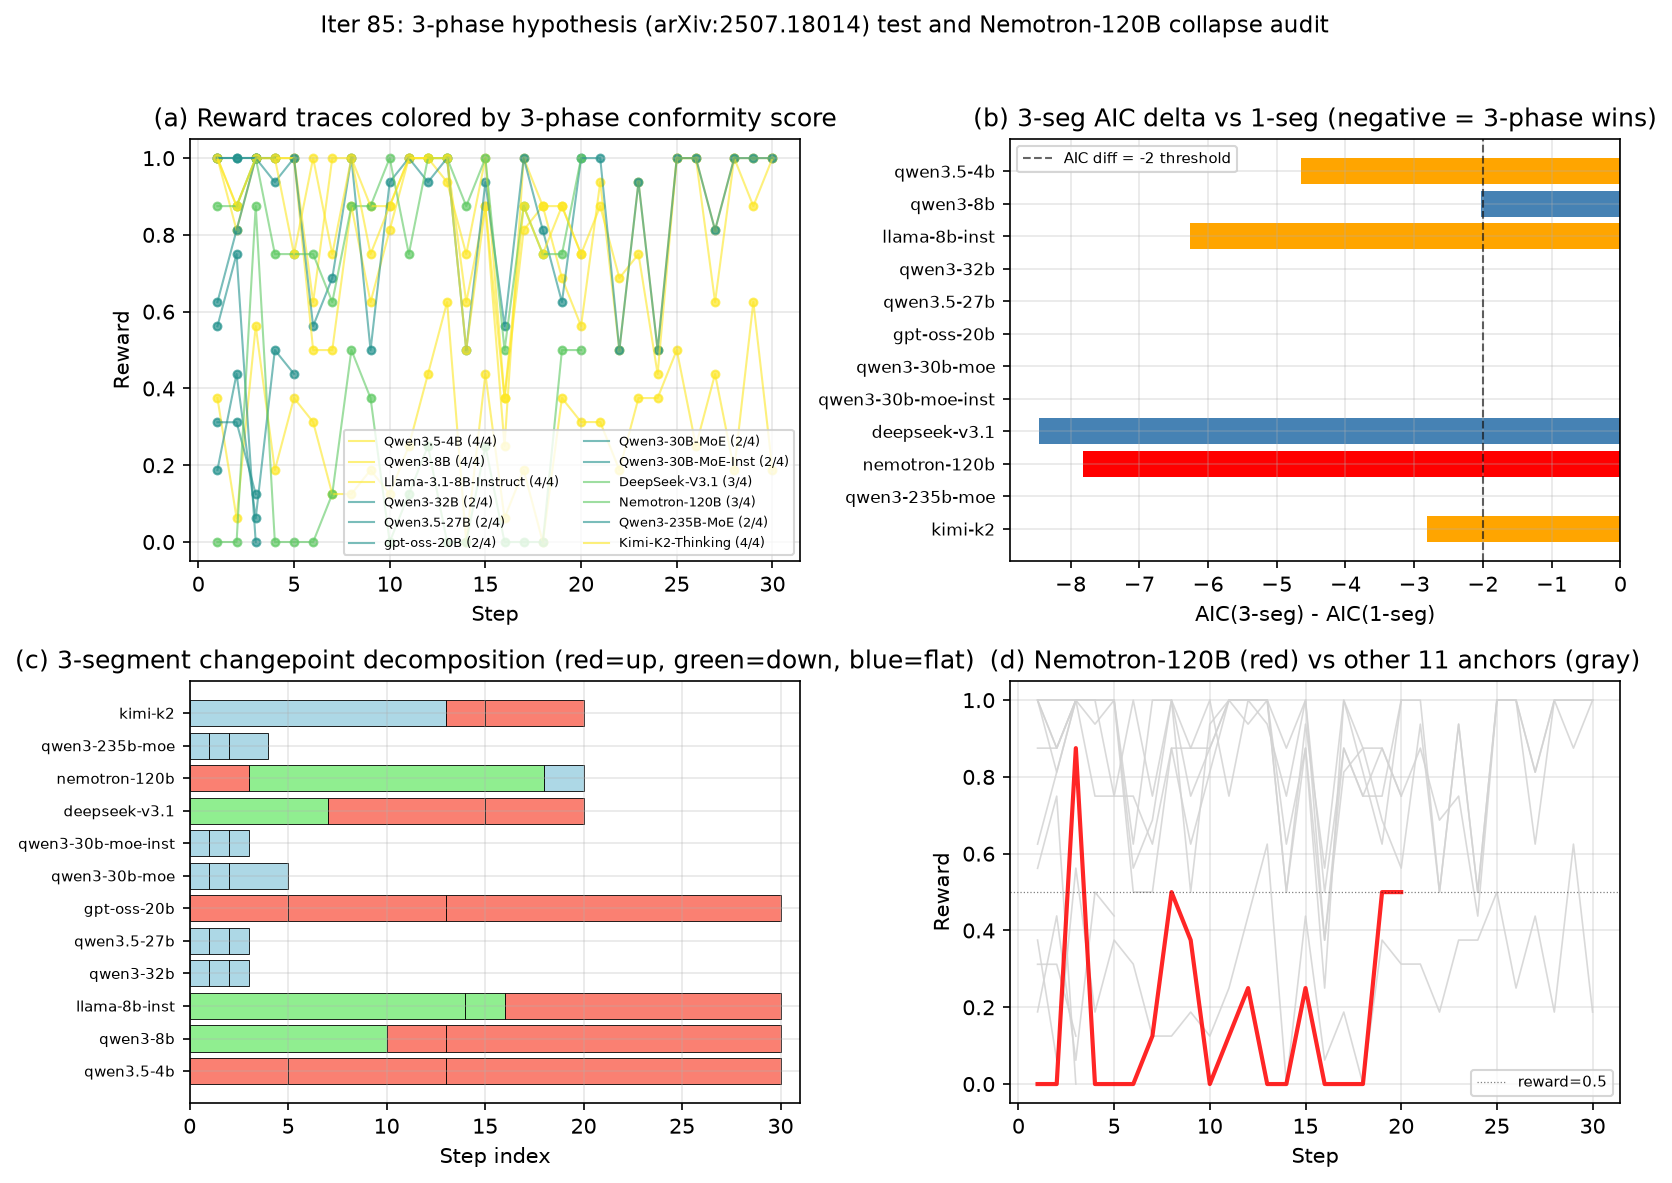
\includegraphics[width=\textwidth]{figures/scaling_law_iter85.pdf}
\caption{Four-panel iter-85 diagnostic. (a) Reward traces for all 12
anchors, colored by 3-phase conformity score ($0$ = purple, $4$ =
yellow).  (b) Horizontal bar chart of $\Delta\mathrm{AIC}_{3\to 1}$ per
anchor; red = collapse label, orange = drift, steelblue = plateau.
(c) 3-segment changepoint decomposition per anchor: red = positive
slope, green = negative slope, lightblue = near-zero slope.  (d)
Nemotron-120B (red) vs.\ the other 11 anchors (gray) -- the early
peak at step 3 and the long collapse to $\sim 0$ are unique.}
\label{fig:iter85}
\end{figure}